\setAuthor{}
\setRound{piirkonnavoor}
\setYear{2019}
\setNumber{G 5}
\setDifficulty{5}
\setTopic{TODO}

\prob{Osake magnetväljas}
\begin{wrapfigure}[7]{r}{0.4\textwidth}
	\vspace{-15pt}
	\begin{center}
		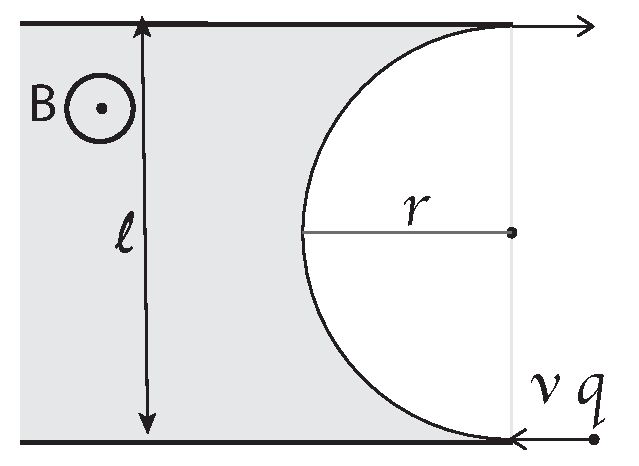
\includegraphics[width = 0.4\textwidth]{2019-v2g-05-yl.pdf}
	\end{center}
\end{wrapfigure}


Osake laenguga $q$ ja massiga $m$ liigub kiirusega $v$ ning siseneb  magnetvälja induktsiooniga $B$. Kui lai peab minimaalselt olema magnetvälja ala $l$, et osake liiguks pärast magnetväljast väljumist esialgsele liikumissuunale vastassuunas?





\hint

\solu
Kui osake siseneb magnetvälja, siis mõjub osakesele Lorenzi jõud $F_L = qvB\sin{\alpha}$ \pp{1}. Osake siseneb magnetvälja risti magnetväljaga ning hakkab Lorentzi jõi tõttu liikuma mööda ringjoont. \pp{2}

Ringjoone raadius $r$ on minimaalne siis, kui osake siseneb magnetvälja alt ning väljub ülevalt servast. Mööda ringjoont liikudes mõjub osakesele tsentrifugaaljõud
\[ F_T = \frac{mv^2}{r} \quad\quad\pp{1} \]
Lorentzi jõud ja tsentrifugaaljõud on võrdsed \pp{1}, seega saame avaldada ringjoone raadiuse $r$
\[ F_L = F_T \quad\quad\Rightarrow\quad\quad qvB = \frac{mv^2}{r} \quad\quad\Rightarrow\quad\quad r = \frac{mv^2}{qvB} \quad\quad\pp{2}\]
Seega on magnetvälja ala minimaalne laius $l$
\[ l = 2r = \frac{2mv^2}{qvB} \quad\quad\pp{1} \]

 \vspace{-20pt}
  \begin{center}
    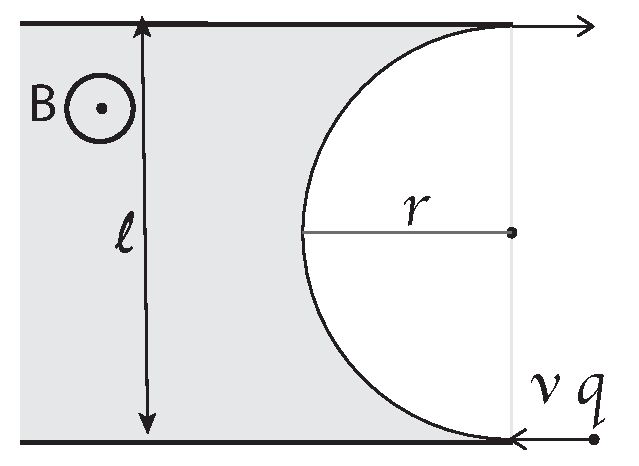
\includegraphics[width=0.5\textwidth]{2019-v2g-05-yl.pdf}
  \end{center}
  \vspace{-20pt}
\probend